\section{State and server-dependent model}\label{sec:state_server_dependent_model}

In addition, the final variation of the queueing model is one that is both
state and server-dependent.
That is, for each server and for each state there is a different service rate.
In other words, each server can have a different service rate for every
possible scenario that the system can be in.

The new service rate \(\mu\) that will be used in this scenario is defined as
a combination of equations~\eqref{eq:state_dependent_service_rate}
and~\eqref{eq:server_dependent_service_rate} where:

\begin{equation}\label{eq:state_server_dependent_service_rate}
    \mu =
    \begin{cases}
        \mu_{1, (0,0)}, & \text{for server } 1 \text{ if } (u, v) = (0, 0) \\
        \mu_{1, (0,1)}, & \text{for server } 1 \text{ if } (u, v) = (0, 1) \\
        \quad \vdots & \qquad \qquad \vdots \\
        \mu_{1, (M,N)}, & \text{for server } 1 \text{ if } (u, v) = (M, N) \\
        \mu_{2, (0,0)}, & \text{for server } 2 \text{ if } (u, v) = (0, 0) \\
        \mu_{2, (0,1)}, & \text{for server } 1 \text{ if } (u, v) = (0, 1) \\
        \quad \vdots & \qquad \qquad \vdots \\
        \mu_{2, (M,N)}, & \text{for server } 2 \text{ if } (u, v) = (M, N) \\
        \quad \vdots & \qquad \qquad \vdots \\
        \mu_{C, (0,0)}, & \text{for server } C \text{ if } (u, v) = (0, 0) \\
        \mu_{C, (0,1)}, & \text{for server } C \text{ if } (u, v) = (0, 1) \\
        \quad \vdots & \qquad \qquad \vdots \\
        \mu_{C, (M,N)}, & \text{for server } C \text{ if } (u, v) = (M, N)
    \end{cases}
\end{equation}

Consider an example where the number of servers is set to \(C = 2\), the
threshold is set to \(T = 1\), node 1 capacity is \(N = 3\) and node 2 capacity
is \(M = 1\).
For this particular example the possible values that \(\mu\) can take shown
by equation~\eqref{eq:state_server_dependent_service_rate_example}.

\begin{equation}\label{eq:state_server_dependent_service_rate_example}
    \mu =
    \begin{cases}
        \mu_{1, (0,0)}, & \text{for server } 1 \text{ if } (u, v) = (0, 0) \\
        \mu_{1, (0,1)}, & \text{for server } 1 \text{ if } (u, v) = (0, 1) \\
        \mu_{1, (0,2)}, & \text{for server } 1 \text{ if } (u, v) = (0, 2) \\
        \mu_{1, (0,3)}, & \text{for server } 1 \text{ if } (u, v) = (0, 3) \\
        \mu_{1, (1,0)}, & \text{for server } 1 \text{ if } (u, v) = (1, 0) \\
        \mu_{1, (1,1)}, & \text{for server } 1 \text{ if } (u, v) = (1, 1) \\
        \mu_{1, (1,2)}, & \text{for server } 1 \text{ if } (u, v) = (1, 2) \\
        \mu_{1, (1,3)}, & \text{for server } 1 \text{ if } (u, v) = (1, 3) \\
        \mu_{2, (0,0)}, & \text{for server } 2 \text{ if } (u, v) = (0, 0) \\
        \mu_{2, (0,1)}, & \text{for server } 2 \text{ if } (u, v) = (0, 1) \\
        \mu_{2, (0,2)}, & \text{for server } 2 \text{ if } (u, v) = (0, 2) \\
        \mu_{2, (0,3)}, & \text{for server } 2 \text{ if } (u, v) = (0, 3) \\
        \mu_{2, (1,0)}, & \text{for server } 2 \text{ if } (u, v) = (1, 0) \\
        \mu_{2, (1,1)}, & \text{for server } 2 \text{ if } (u, v) = (1, 1) \\
        \mu_{2, (1,2)}, & \text{for server } 2 \text{ if } (u, v) = (1, 2) \\
        \mu_{2, (1,3)}, & \text{for server } 2 \text{ if } (u, v) = (1, 3)
    \end{cases}
\end{equation}


\subsection{Implementation}

The implementation of the state and server-dependent model is the
combination of the state-dependent and server-dependent models' implementation.
Once again the implementation is done using the python library \(\texttt{ciw}\)
library.
The distribution for the state and server-dependent model is defined as a
class that inherits from \texttt{ciw}'s class \texttt{Distribution} from
the \texttt{dists} module.
Note that as opposed to the classes defined earlier an additional method id
defined in this class.
Method \texttt{update\_server\_attributes} adds additional attributes to the
server objects to allow for further analysis of each server's performance.

\begin{lstlisting}[
    style=pystyle,
    caption={Example of the state and server-dependent variation of the
    queueing system},
    label={lst:state_server_dependent_example},
]
>>> import random
>>> import ciw
>>> class StateServerDependentExponential(
...     ciw.dists.Distribution
... ):
...     def __init__(self, rates):
...         self.simulation = None
...         self.rates = rates
... 
...     def sample(self, t=None, ind=None):
...         """
...         This method is used to sample the service time for an individual
...         based on the current state and the server that the individual is
...         assigned to. The following steps are being taken:
...             1. Find the server
...             2. Find the state
...             3. Check if the state is valid. Note that there are some cases
...                 where the visited state is not valid. These are the cases
...                 where the state `(u, T-1)` is visited where `u > 0`. This
...                 is meant to be an unreachable state. In such case remap
...                 the state to `(u+1, T)`
...             4. Get the service rate for that server and state
...             5. Sample the service time
...             6. Update any possible attributes for the server
...         """
...         server = ind.server.id_number
...         state = (
...             len(ind.simulation.nodes[1].individuals[0]),
...             len(ind.simulation.nodes[2].individuals[0]),
...         )
...         is_invalid = state[0] > 0 and state[1] < ind.simulation.threshold
...         if is_invalid:
...             state = (state[0] - 1, state[1] + 1)
...         rate = self.rates[server][state]
...         service_time = random.expovariate(rate)
...         self.update_server_attributes(ind, service_time)
...         return service_time
... 
...     def update_server_attributes(self, ind, service_time):
...         """
...         Updates the server's attributes
...         """
...         if hasattr(ind.server, "served_inds"):
...             ind.server.served_inds.append(self.simulation.current_time)
...         else:
...             ind.server.served_inds = [self.simulation.current_time]
... 
...         if hasattr(ind.server, "service_times"):
...             ind.server.service_times.append(service_time)
...         else:
...             ind.server.service_times = [service_time]

\end{lstlisting}

Now consider an example where the number of servers is set to \(C = 2\), the
threshold is set to \(T = 1\), node 1 capacity is \(N = 3\) and node 2 capacity
is \(M = 1\).
Let the service rates be defined in such a way where:

\begin{enumerate}
    \item Server 1's service rate is \(0.5\) whenever there are less than two
    individuals in the entire system, otherwise the service rate is \(1\).
    \item Server 2's service rate is \(0.7\) whenever there are less than three
    individuals in the entire system, otherwise the service rate is \(1.5\).
\end{enumerate}

The following code snippet shows how to define the model and run the simulation
for \(1000\) time units.

\begin{lstlisting}[
    style=pystyle,
    caption={Example code of the state and server-dependent variation of the
    queueing system},
    label={lst:state_server_dependent_example_code},
]
>>> import ambulance_game as abg
>>> import numpy as np
>>>
>>> lambda_1 = 1
>>> lambda_2 = 1
>>> num_of_servers = 2
>>> threshold = 1
>>> system_capacity = 3
>>> buffer_capacity = 1
>>> runtime = 1000
>>> seed_num = 0
>>> 
>>> all_states = abg.markov.build_states(
...     threshold=threshold,
...     system_capacity=system_capacity,
...     buffer_capacity=buffer_capacity
... )
>>> mu = {k: {} for k in range(1, num_of_servers + 1)}
>>> mu[1] = {(u, v): 0.5 if u + v < 2 else 1 for u, v in all_states}
>>> mu[2] = {(u, v): 0.7 if u + v < 3 else 1.5 for u, v in all_states}
>>>
>>> Q = abg.simulation.simulate_model(
...     lambda_1=lambda_1,
...     lambda_2=lambda_2,
...     mu=mu,
...     num_of_servers=num_of_servers,
...     threshold=threshold,
...     seed_num=seed_num,
...     system_capacity=system_capacity,
...     buffer_capacity=buffer_capacity,
...     runtime=runtime,
... )
>>> for srv, mean_service_time in enumerate([
...     np.round(np.mean(s.service_times), 8)
...     for s in Q.nodes[2].servers
... ]):
...     print(f"Server {srv + 1}:", mean_service_time)
Server 1: 1.79718861
Server 2: 0.87253758

\end{lstlisting}

Note that, in the implementation shown in code
snippet~\ref{lst:state_server_dependent_example_code} the individuals are
paired with a server
in an ``unfair'' way since the default behaviour of \texttt{ciw} does not
focus on the fairness of server allocation.
Server 1 is always assigned an individual if they are free, while Server 2 is
only assigned an individual if Server 1 is busy.
For the purposes of this project though, it is important to have a more
``fair'' allocation of individuals to servers.
This can be done by using the \texttt{server\_priority\_function} argument of
the \texttt{simulate\_model} function.

\begin{lstlisting}[
    style=pystyle,
    caption={Example of using fair allocation of individuals to servers},
    label={lst:fair_allocation_example_code},
]
>>> Q = abg.simulation.simulate_model(
...     lambda_1=lambda_1,
...     lambda_2=lambda_2,
...     mu=mu,
...     num_of_servers=num_of_servers,
...     threshold=threshold,
...     seed_num=seed_num,
...     system_capacity=system_capacity,
...     buffer_capacity=buffer_capacity,
...     runtime=runtime,
...     server_priority_function=lambda srv, ind: random.random()
... )
>>> for srv, mean_service_time in enumerate([
...     np.round(np.mean(s.service_times), 8)
...     for s in Q.nodes[2].servers
... ]):
...     print(f"Server {srv + 1}:", mean_service_time)
Server 1: 1.31071177
Server 2: 1.02142722

\end{lstlisting}


\subsection{Game theoretic model}

The state and server dependent model can be used in the game theoretic
model described from Section~\ref{sec:game_theoretic_model}.
However, since the state and server dependent model variant of the queueing
theoretic model is only implemented using Discrete Event Simulation (DES), it is
not possible to use the Markov chain model here.
Thus, the implementation of the game was modified so that it can be used with
the DES model as well.
More details on the code can be found in
Appendix~\ref{appendix:ambulance_game}.
At its core, the only metric that is needed from the Markov model are the
performance measures of the queue (blocking time and proportion of individuals
within target) which can also be obtained using the DES model.
Consequently, the payoff matrices can be calculated using these performance
measures.

Something that needs to be taken into consideration here is whether the results
of the game are the same when using the DES model and the Markov chain model.
In fact using the DES approach, several other parameters are introduced that
can affect the results of the game.
Such parameters are the runtime, the warm up time and the cooldown time of the
simulation.
The runtime of the simulation is the total time that the simulation is run for,
the warm up time is the time that the simulation is run for before the
data collection starts and the cooldown time is the time that the simulation is
run for after the data collection has finished.
The runtime of the simulation is the parameter that is most likely to affect
the performance measures of the queue, since the longer the simulation is run
for, the better the estimates of the performance measures will be.

Consider a game with the parameters shown in
Table~\ref{tab:game_with_des_parameters}.

\begin{table}[H]
    \caption{Parameter values for game theoretic model example to observe the
    differences of running the game with DES and Markov chains.}
    \begin{center}
        \begin{tabular}{||c|c|c|c||c|c|c|c|c||c|c|c|c|c||}
            \hline
            \multicolumn{4}{||c||}{\textbf{Distributor}} &
            \multicolumn{5}{c||}{\textbf{Queueing system \(A\)}} &
            \multicolumn{5}{c||}{\textbf{Queueing system \(B\)}} \\
            \hline
            \(\lambda_2\) & t & \footnotesize{\(\hat{P}\)} & \(\alpha\) &
            \(\lambda_1^A\) & \(\mu^A\) & \(C^A\) & \(N^A\) & \(M^A\) &
            \(\lambda_1^B\) & \(\mu^B\) & \(C^B\) & \(N^B\) & \(M^B\) \\
            \hline
            2 & 2 & 0.95 & 0.2 & 2 & 2 & 2 & 6 & 2 & 2 & 2 & 2 & 6 & 2 \\
            \hline
        \end{tabular}
    \end{center}
    \label{tab:game_with_des_parameters}
\end{table}

For a complete description of parameter notations see
Section~\ref{sec:game_players_and_parameters}.
Figure~\ref{fig:game_des_markov_baseline} shows the asymmetric replicator
dynamics run of the game when the payoff matrices are calculated using the
Markov chain model.

\begin{figure}[ht]
    \centering
    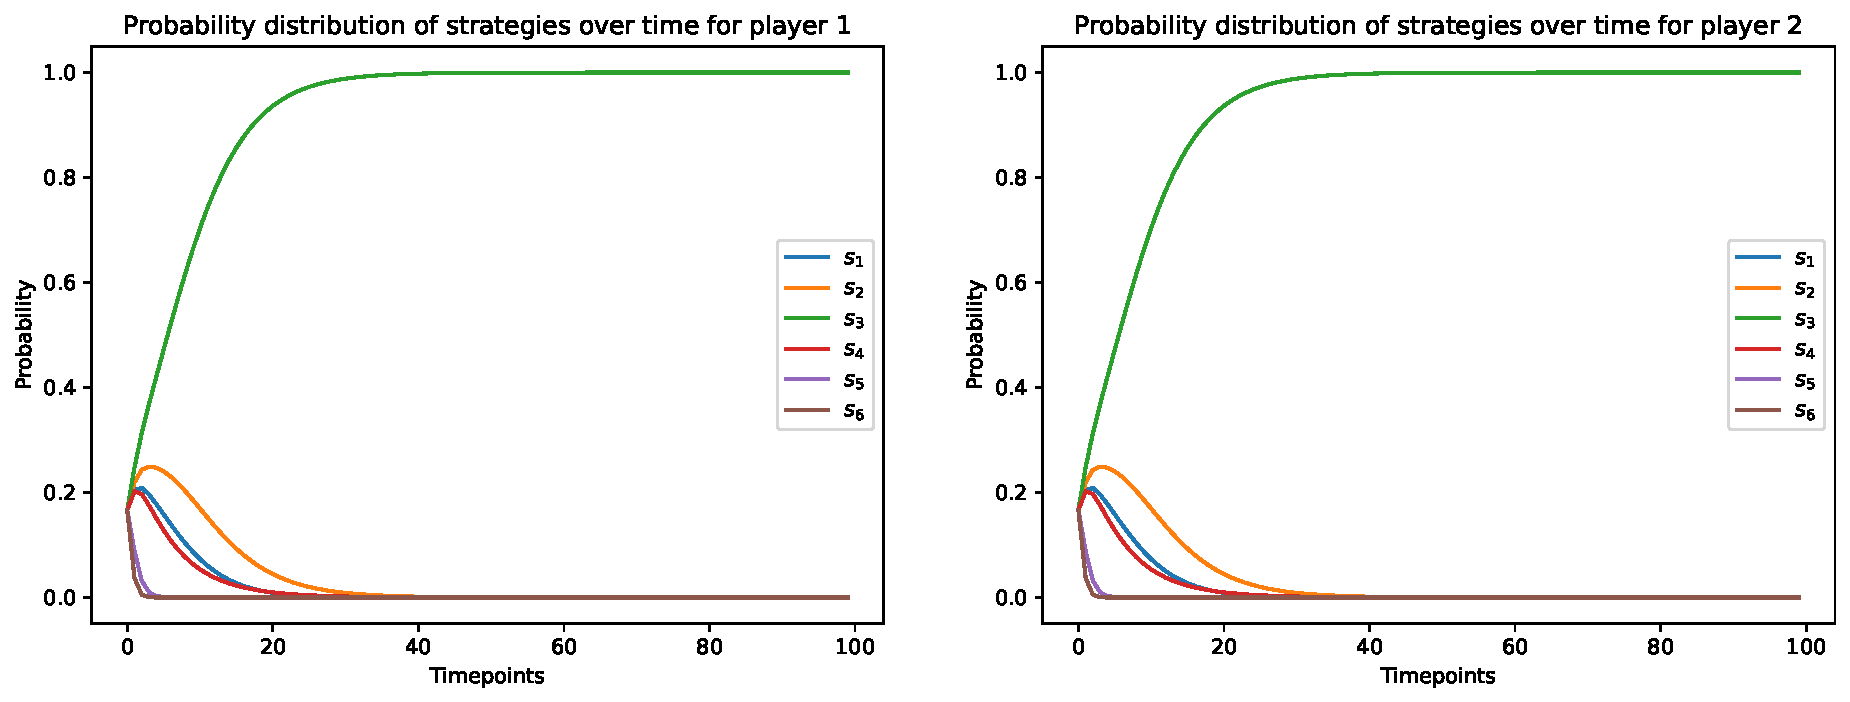
\includegraphics[width=0.8\textwidth]{chapters/06_agent_based_extension/Bin/game_model_with_des/game_markov_baseline.pdf}
    \caption{Asymmetric replicator dynamics algorithm run on the game obtained
    from the Markov chain model.}
    \label{fig:game_des_markov_baseline}
\end{figure}

It can be seen that both player end up playing strategy \(s_3\) which
corresponds to choosing a threshold of \(T^{(A)} = 3\) and \(T^{(B)} = 3\).
Figures~\ref{fig:game_des_runtime_300}, \ref{fig:game_des_runtime_500} and
\ref{fig:game_des_runtime_1000} show the asymmetric replicator dynamics run of
the game when the payoff matrices are calculated using the DES model with
different runtimes.
More specifically, the runtime of the DES model is set to \(300\), \(500\) and
\(1000\) time units respectively.

\begin{figure}[H]
    \centering
    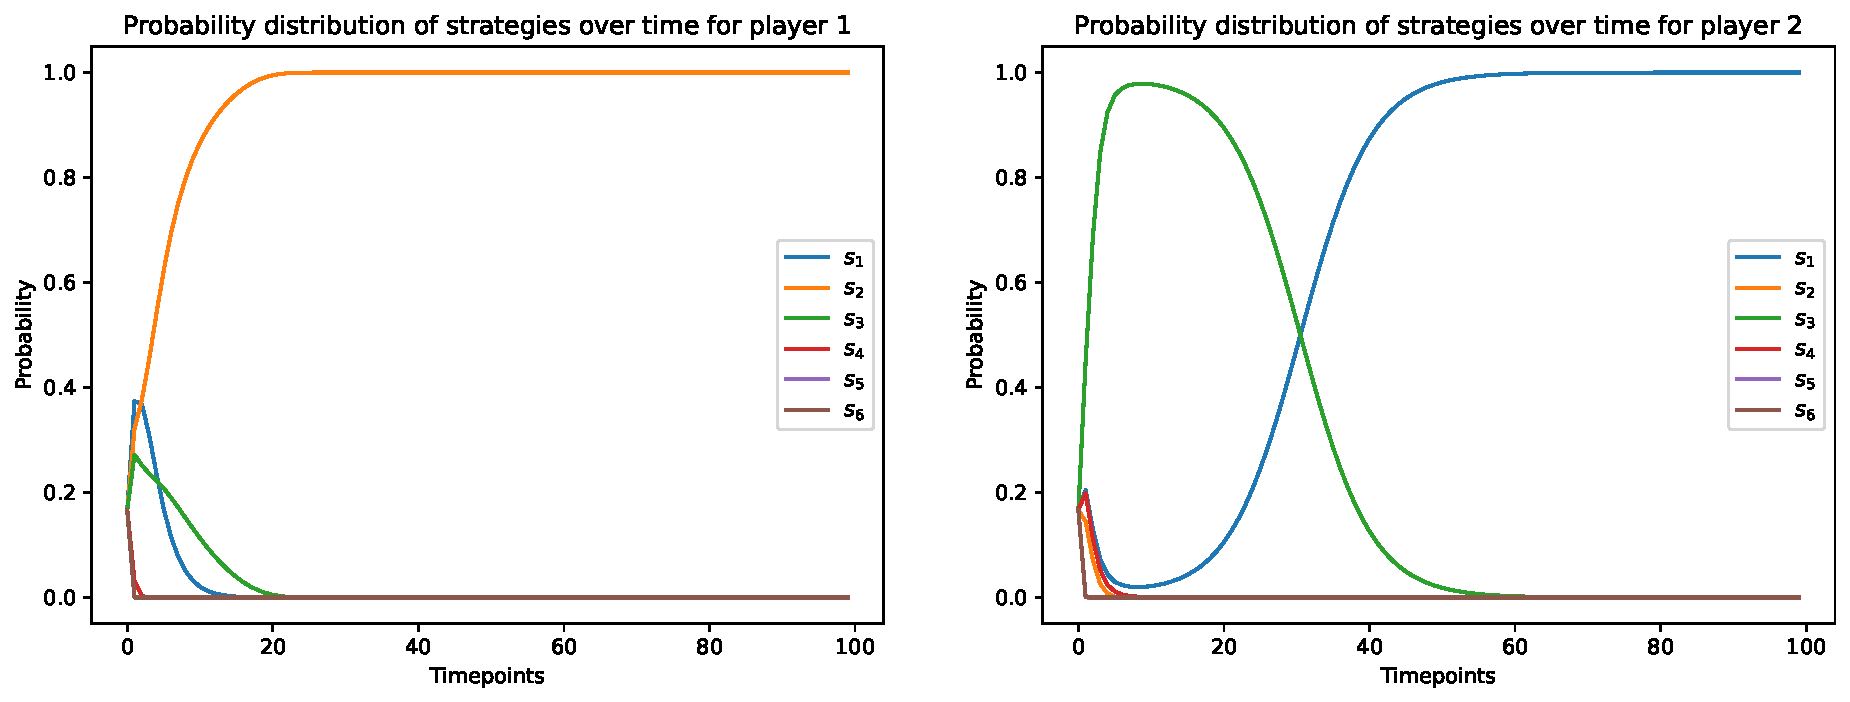
\includegraphics[width=0.8\textwidth]{chapters/06_agent_based_extension/Bin/game_model_with_des/game_simulation_300.pdf}
    \caption{Asymmetric replicator dynamics algorithm run on the game obtained
    from the DES model using a runtime of \(300\) time units.}
    \label{fig:game_des_runtime_300}
\end{figure}

\begin{figure}[H]
    \centering
    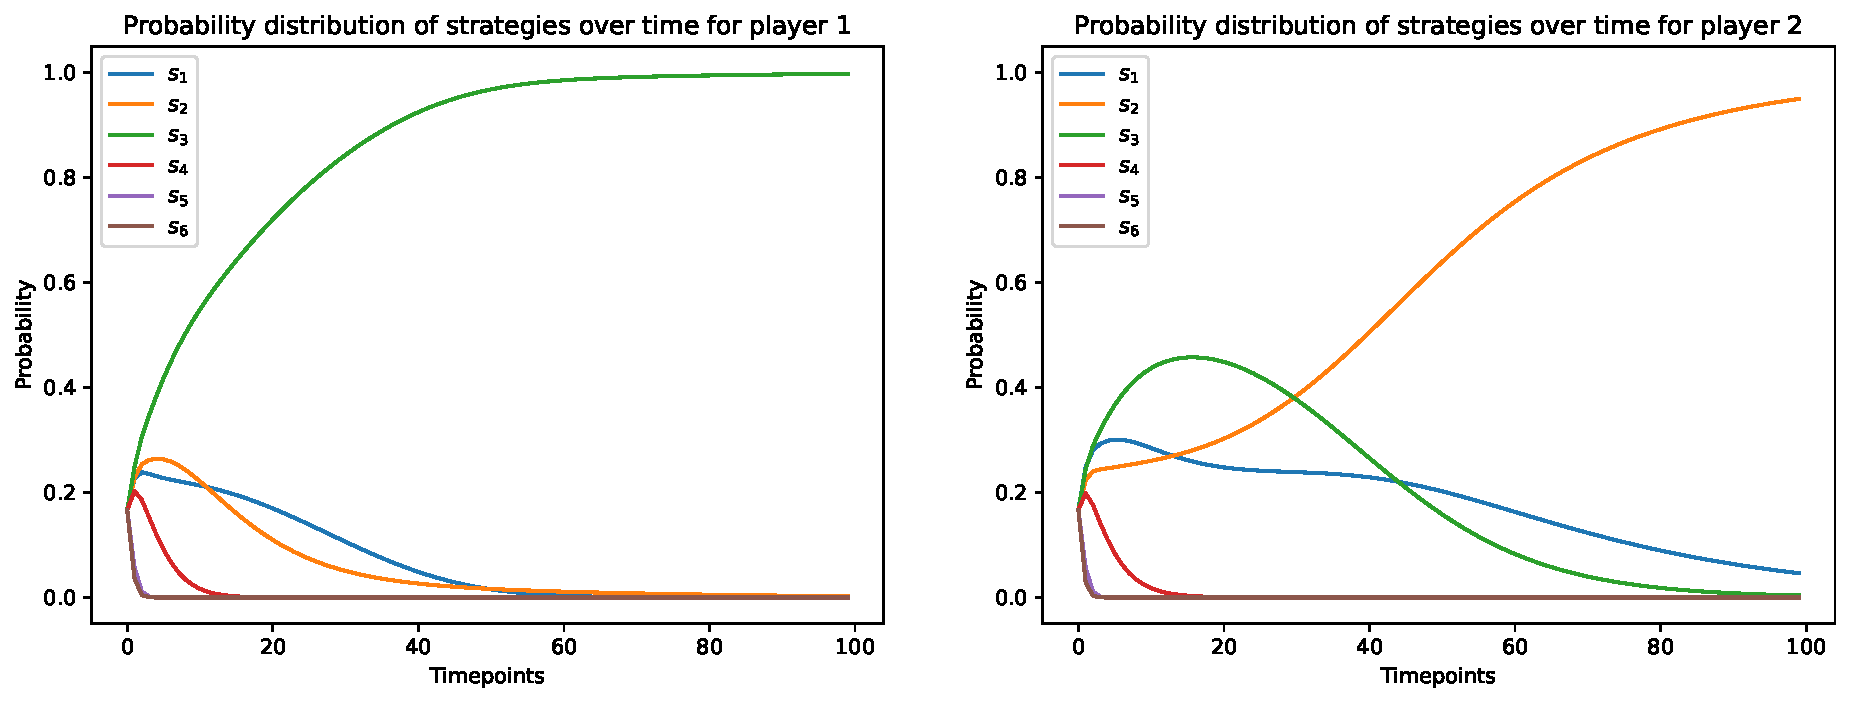
\includegraphics[width=0.8\textwidth]{chapters/06_agent_based_extension/Bin/game_model_with_des/game_simulation_500.pdf}
    \caption{Asymmetric replicator dynamics algorithm run on the game obtained
    from the DES model using a runtime of \(500\) time units.}
    \label{fig:game_des_runtime_500}
\end{figure}

\begin{figure}[H]
    \centering
    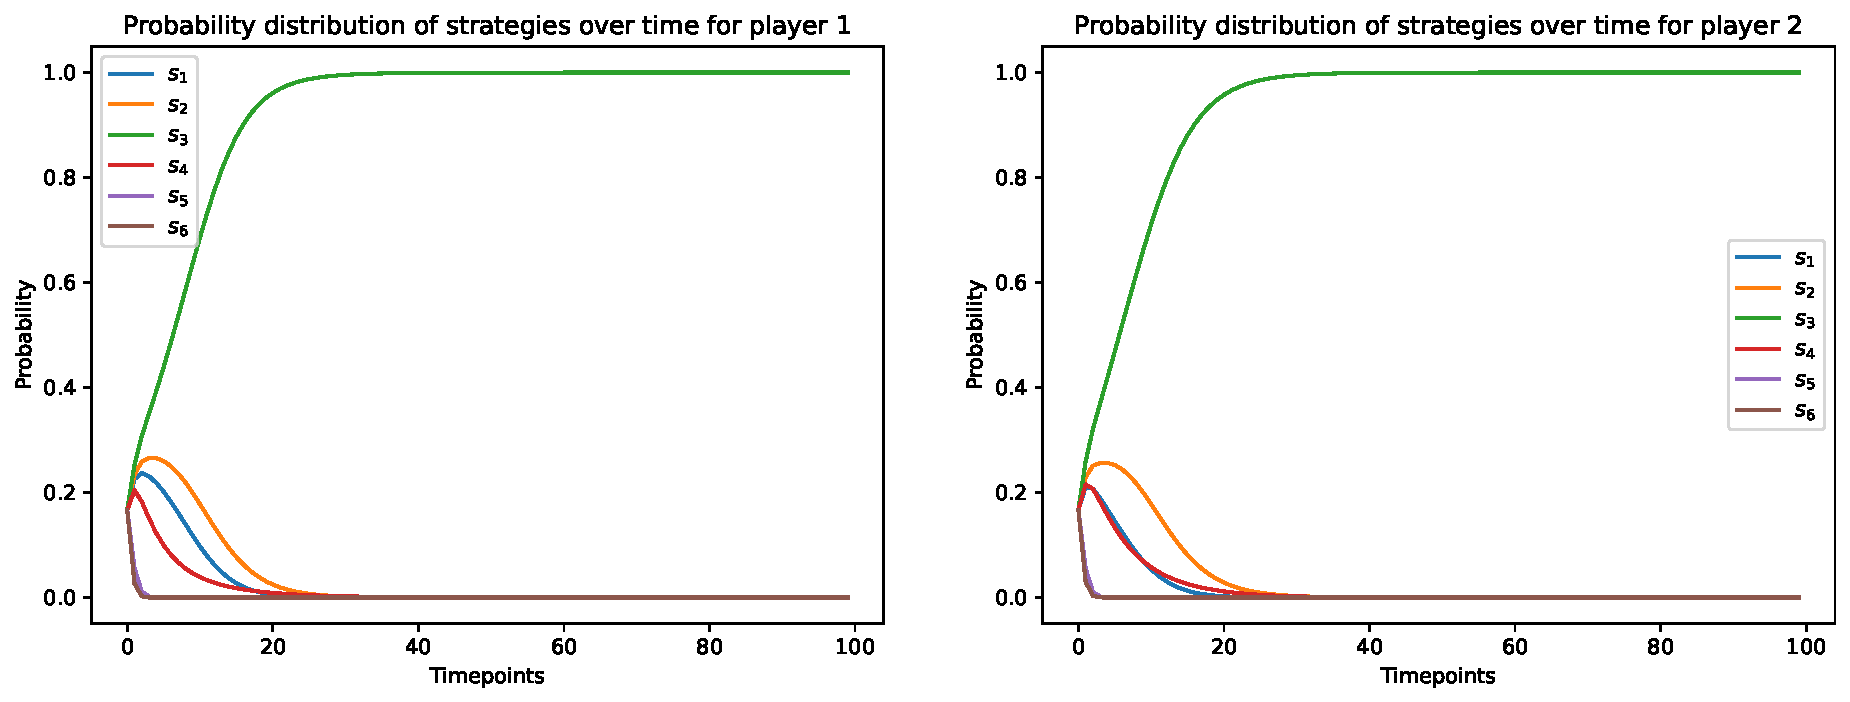
\includegraphics[width=0.8\textwidth]{chapters/06_agent_based_extension/Bin/game_model_with_des/game_simulation_1000.pdf}
    \caption{Asymmetric replicator dynamics algorithm run on the game obtained
    from the DES model using a runtime of \(1000\) time units.}
    \label{fig:game_des_runtime_1000}
\end{figure}

By observing the asymmetric replicator dynamics run of the game with the DES
model when using different runtimes, it can be noticed that the results from
using a runtime of \(300\) time units and a runtime of \(500\) time units are
different from the ones obtained using the Markov chain model.
However, the resultant strategies from using a runtime of \(1000\) time units
are the same as the ones obtained using the Markov chain model.
This is due to the fact that the runtime of the DES model needs to be long
enough for the simulation to reach a steady state.
For this particular example, it seems that a runtime of \(1000\) time units is
sufficient.


Having found a reasonable runtime for the DES model, the state and server
dependent distribution of the service rate can be used in the game theoretic
model.
Consider a small change to the parameter values defined earlier, where the
service rate is now state and server dependent.
Let the service rate for queueing system \(1\) be \(\mu^{(1)} = 6\) only for
server \(1\) if there are \(4\) or more individuals in the system
and \(\mu^{(1)} = 2\) otherwise.
Additionally, let the service rate for queueing system \(2\) be
\(\mu^{(2)} = 8\) only for server \(1\) if there are \(3\) or more
individuals in node 1 and \(\mu^{(2)} = 2\) otherwise.
In other words the service rate is now defined as:

\begin{align}
    \mu^{(1)} =
    \begin{cases}
        6, & \text{if server id \(= 1\) and } u_1 + v_1 \geq 4 \\
        2, & \text{otherwise}
    \end{cases} \\
    \mu^{(2)} =
    \begin{cases}
        8, & \text{if server id \(= 1\) and } u_1 \geq 3 \\
        2, & \text{otherwise}
    \end{cases}
\end{align}

The game theoretic model is then run using the DES model with a runtime of
\(3000\) time units.
Figure~\ref{fig:game_server_state_dependen_example} shows the asymmetric
replicator dynamics run of the game when the payoff matrices are calculated
using the DES model with this new service rate distribution.

\begin{figure}[H]
    \centering
    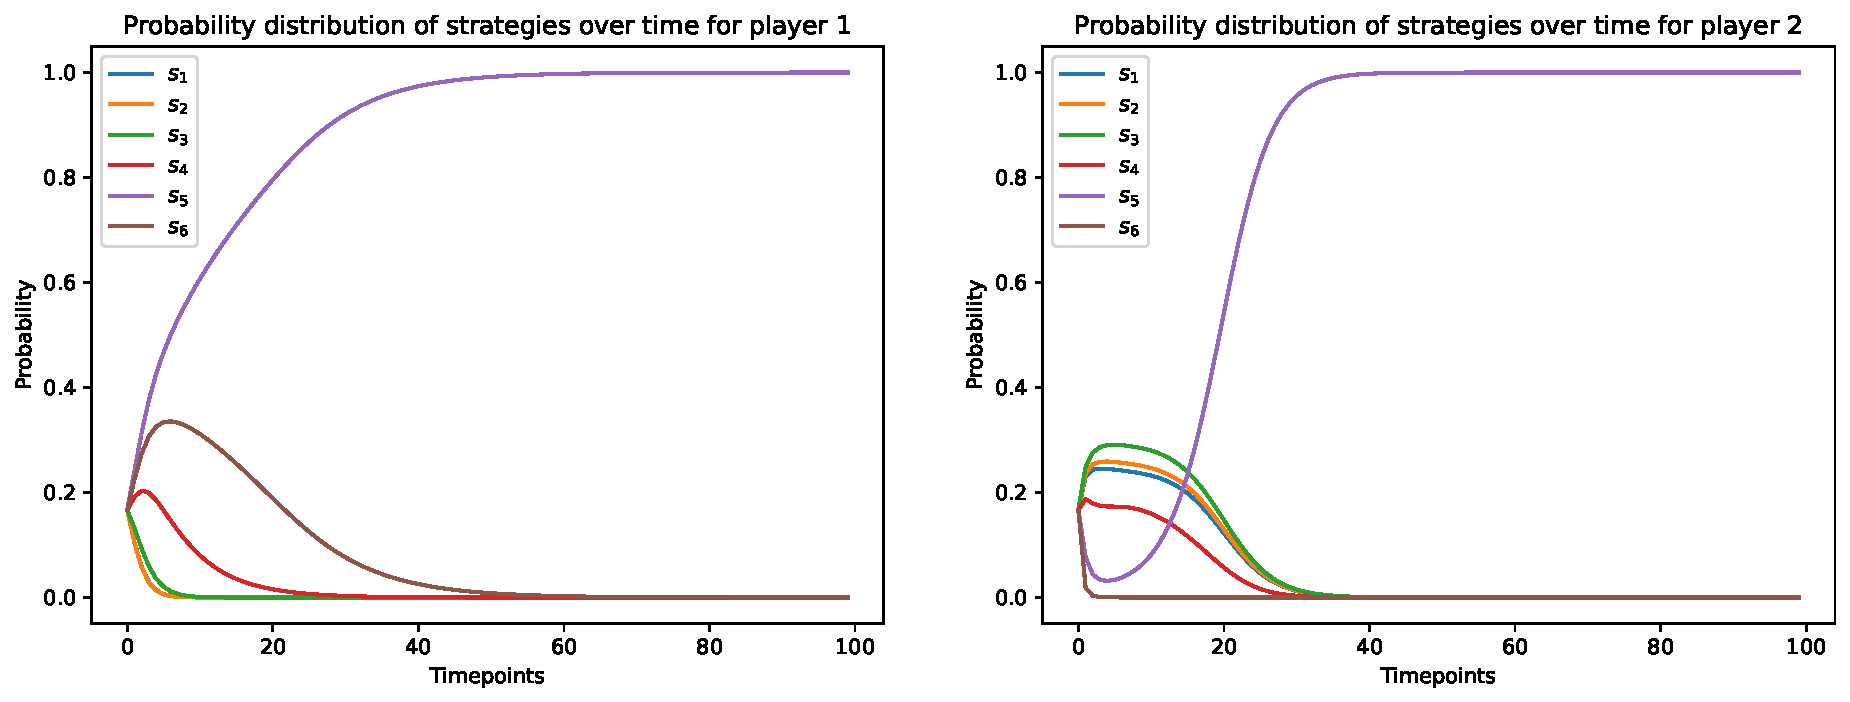
\includegraphics[width=0.8\textwidth]{chapters/06_agent_based_extension/Bin/game_model_with_des/game_server_state_dependent_3000.pdf}
    \caption{Asymmetric replicator dynamics algorithm run on the game obtained
    from the DES model using a runtime of \(3000\) time units and a state and
    server dependent service rate.}
    \label{fig:game_server_state_dependen_example}
\end{figure}

It can be seen that the outcome of the game is different than before.
Player \(1\) chooses to play strategy \(s_5\) and player \(2\) also ends up
playing strategy \(s_5\).
That corresponds to choosing a threshold of \(T^{(1)} = 5\) and a threshold of
\(T^{(2)} = 5\).
The change in the service distribution made server \(1\) of queueing system
\(1\) and server \(1\) of queueing system \(2\) work faster when their
corresponding system was getting busier.
This change in the service rate distribution made the queueing systems
increase their thresholds in the game, and thus block less type \(2\)
individuals at node \(1\).
Refer to Figure~\ref{fig:diagram_of_queueing_system} for a visual
representation of the types of individuals and the nodes of the queueing
systems. 

